% GNUPLOT: LaTeX picture with Postscript
\begingroup
  \fontfamily{Arial}%
  \selectfont
  \makeatletter
  \providecommand\color[2][]{%
    \GenericError{(gnuplot) \space\space\space\@spaces}{%
      Package color not loaded in conjunction with
      terminal option `colourtext'%
    }{See the gnuplot documentation for explanation.%
    }{Either use 'blacktext' in gnuplot or load the package
      color.sty in LaTeX.}%
    \renewcommand\color[2][]{}%
  }%
  \providecommand\includegraphics[2][]{%
    \GenericError{(gnuplot) \space\space\space\@spaces}{%
      Package graphicx or graphics not loaded%
    }{See the gnuplot documentation for explanation.%
    }{The gnuplot epslatex terminal needs graphicx.sty or graphics.sty.}%
    \renewcommand\includegraphics[2][]{}%
  }%
  \providecommand\rotatebox[2]{#2}%
  \@ifundefined{ifGPcolor}{%
    \newif\ifGPcolor
    \GPcolorfalse
  }{}%
  \@ifundefined{ifGPblacktext}{%
    \newif\ifGPblacktext
    \GPblacktexttrue
  }{}%
  % define a \g@addto@macro without @ in the name:
  \let\gplgaddtomacro\g@addto@macro
  % define empty templates for all commands taking text:
  \gdef\gplbacktext{}%
  \gdef\gplfronttext{}%
  \makeatother
  \ifGPblacktext
    % no textcolor at all
    \def\colorrgb#1{}%
    \def\colorgray#1{}%
  \else
    % gray or color?
    \ifGPcolor
      \def\colorrgb#1{\color[rgb]{#1}}%
      \def\colorgray#1{\color[gray]{#1}}%
      \expandafter\def\csname LTw\endcsname{\color{white}}%
      \expandafter\def\csname LTb\endcsname{\color{black}}%
      \expandafter\def\csname LTa\endcsname{\color{black}}%
      \expandafter\def\csname LT0\endcsname{\color[rgb]{1,0,0}}%
      \expandafter\def\csname LT1\endcsname{\color[rgb]{0,1,0}}%
      \expandafter\def\csname LT2\endcsname{\color[rgb]{0,0,1}}%
      \expandafter\def\csname LT3\endcsname{\color[rgb]{1,0,1}}%
      \expandafter\def\csname LT4\endcsname{\color[rgb]{0,1,1}}%
      \expandafter\def\csname LT5\endcsname{\color[rgb]{1,1,0}}%
      \expandafter\def\csname LT6\endcsname{\color[rgb]{0,0,0}}%
      \expandafter\def\csname LT7\endcsname{\color[rgb]{1,0.3,0}}%
      \expandafter\def\csname LT8\endcsname{\color[rgb]{0.5,0.5,0.5}}%
    \else
      % gray
      \def\colorrgb#1{\color{black}}%
      \def\colorgray#1{\color[gray]{#1}}%
      \expandafter\def\csname LTw\endcsname{\color{white}}%
      \expandafter\def\csname LTb\endcsname{\color{black}}%
      \expandafter\def\csname LTa\endcsname{\color{black}}%
      \expandafter\def\csname LT0\endcsname{\color{black}}%
      \expandafter\def\csname LT1\endcsname{\color{black}}%
      \expandafter\def\csname LT2\endcsname{\color{black}}%
      \expandafter\def\csname LT3\endcsname{\color{black}}%
      \expandafter\def\csname LT4\endcsname{\color{black}}%
      \expandafter\def\csname LT5\endcsname{\color{black}}%
      \expandafter\def\csname LT6\endcsname{\color{black}}%
      \expandafter\def\csname LT7\endcsname{\color{black}}%
      \expandafter\def\csname LT8\endcsname{\color{black}}%
    \fi
  \fi
    \setlength{\unitlength}{0.0500bp}%
    \ifx\gptboxheight\undefined%
      \newlength{\gptboxheight}%
      \newlength{\gptboxwidth}%
      \newsavebox{\gptboxtext}%
    \fi%
    \setlength{\fboxrule}{0.5pt}%
    \setlength{\fboxsep}{1pt}%
\begin{picture}(7200.00,5040.00)%
    \gplgaddtomacro\gplbacktext{%
      \csname LTb\endcsname%%
      \put(576,288){\makebox(0,0)[r]{\strut{}$-0.8$}}%
      \put(576,734){\makebox(0,0)[r]{\strut{}$-0.7$}}%
      \put(576,1181){\makebox(0,0)[r]{\strut{}$-0.6$}}%
      \put(576,1627){\makebox(0,0)[r]{\strut{}$-0.5$}}%
      \put(576,2074){\makebox(0,0)[r]{\strut{}$-0.4$}}%
      \put(576,2520){\makebox(0,0)[r]{\strut{}$-0.3$}}%
      \put(931,1627){\makebox(0,0)[l]{\strut{}$8\uparrow$}}%
      \put(767,1627){\makebox(0,0)[l]{\strut{}$8\downarrow$}}%
      \put(1168,1627){\makebox(0,0)[l]{\strut{}$9\downarrow$}}%
      \put(1379,1627){\makebox(0,0)[l]{\strut{}$9\downarrow$}}%
    }%
    \gplgaddtomacro\gplfronttext{%
      \csname LTb\endcsname%%
      \put(-228,1404){\rotatebox{-270}{\makebox(0,0){\strut{}$E(eV)$}}}%
      \csname LTb\endcsname%%
      \put(1547,2880){\makebox(0,0){\strut{}Left}}%
    }%
    \gplgaddtomacro\gplbacktext{%
      \csname LTb\endcsname%%
      \put(3208,1627){\makebox(0,0)[l]{\strut{}$9\uparrow\downarrow$}}%
      \put(2603,1627){\makebox(0,0)[l]{\strut{}$8\uparrow\downarrow$}}%
    }%
    \gplgaddtomacro\gplfronttext{%
      \csname LTb\endcsname%%
      \put(3563,2880){\makebox(0,0){\strut{}Center}}%
    }%
    \gplgaddtomacro\gplbacktext{%
      \csname LTb\endcsname%%
      \put(5018,1627){\makebox(0,0)[l]{\strut{}$8\uparrow$}}%
      \put(4812,1627){\makebox(0,0)[l]{\strut{}$8\downarrow$}}%
      \put(5317,1627){\makebox(0,0)[l]{\strut{}$9\downarrow$}}%
      \put(5582,1627){\makebox(0,0)[l]{\strut{}$9\uparrow$}}%
    }%
    \gplgaddtomacro\gplfronttext{%
      \csname LTb\endcsname%%
      \put(5795,2880){\makebox(0,0){\strut{}Right}}%
    }%
    \gplgaddtomacro\gplbacktext{%
      \csname LTb\endcsname%%
      \put(576,2760){\makebox(0,0)[r]{\strut{}$-10$}}%
      \put(576,3013){\makebox(0,0)[r]{\strut{}$-8$}}%
      \put(576,3266){\makebox(0,0)[r]{\strut{}$-6$}}%
      \put(576,3520){\makebox(0,0)[r]{\strut{}$-4$}}%
      \put(576,3773){\makebox(0,0)[r]{\strut{}$-2$}}%
      \put(576,4026){\makebox(0,0)[r]{\strut{}$0$}}%
      \put(576,4279){\makebox(0,0)[r]{\strut{}$2$}}%
      \put(576,4533){\makebox(0,0)[r]{\strut{}$4$}}%
      \put(576,4786){\makebox(0,0)[r]{\strut{}$6$}}%
      \put(576,5039){\makebox(0,0)[r]{\strut{}$8$}}%
    }%
    \gplgaddtomacro\gplfronttext{%
      \csname LTb\endcsname%%
      \put(-84,3899){\rotatebox{-270}{\makebox(0,0){\strut{}E(ev)}}}%
      \csname LTb\endcsname%%
      \put(1547,5399){\makebox(0,0){\strut{}Right}}%
    }%
    \gplgaddtomacro\gplbacktext{%
    }%
    \gplgaddtomacro\gplfronttext{%
      \csname LTb\endcsname%%
      \put(3563,5399){\makebox(0,0){\strut{}Right}}%
    }%
    \gplgaddtomacro\gplbacktext{%
    }%
    \gplgaddtomacro\gplfronttext{%
      \csname LTb\endcsname%%
      \put(5795,5399){\makebox(0,0){\strut{}Right}}%
    }%
    \gplbacktext
    \put(0,0){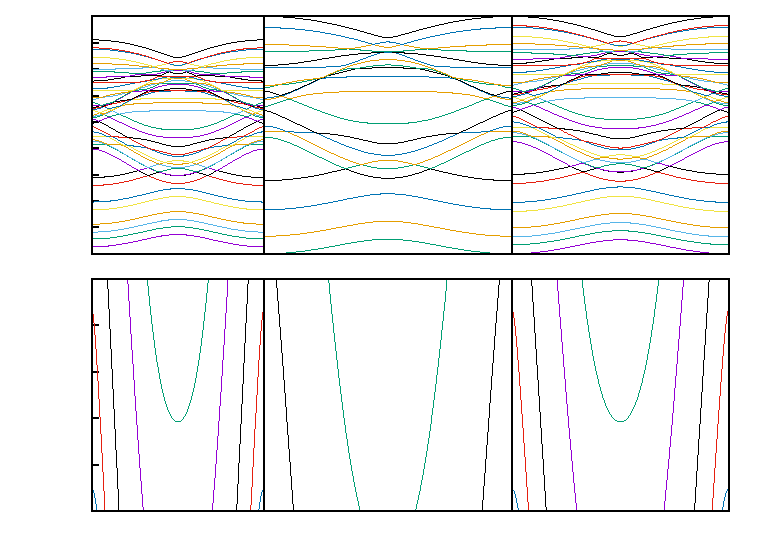
\includegraphics[width={360.00bp},height={252.00bp}]{borophene_band}}%
    \gplfronttext
  \end{picture}%
\endgroup
